%xelatex -shell-escape -output-directory=bin ergasia.tex
\documentclass{assignment}

\usepackage{enumerate} % Για την χρησιμοποίηση roman enumerate
\usepackage{paralist} % για το περιβάλλον inparaenum που είναι οι λίστες μέσα στο κείμενο.

\title{Δίκτυα Υπολογιστών \\ 2ο Εργαστήριο: Δυναμική Δρομολόγηση \\ Εργασία: assign2}
\date{Αθήνα, 2015}

\author{Αναγνωστόπουλος Βασίλης - Θάνος (ΜΠΠΛ 13002) \and Βελισσαρίου Κυριάκος (ΜΠΠΛ 13005)}

\begin{document}

\maketitle
% Να σκεφτώ τί αλλαγές θέλω να κάνω με τις αριθμήσεις και άμα θέλω να κάνω.
% Να σκεφτώ να τις ενσωματώσω και στο assignment.cls

\setcounter{page}{1} 
\pagenumbering{roman}

\pagestyle{plain}
\tableofcontents
\listoftables
\listoffigures
%\renewcommand\listoflistingscaption{Κατάλογος πηγαίου κώδικα}
%\listoflistings
\newpage

%\pagestyle{headings}
%\pagestyle{fancy}
\setcounter{page}{1} 
\pagenumbering{arabic}


Δίνεται η παρακάτω τοπολογία:

\begin{center}
\resizebox*{\textwidth}{!}{
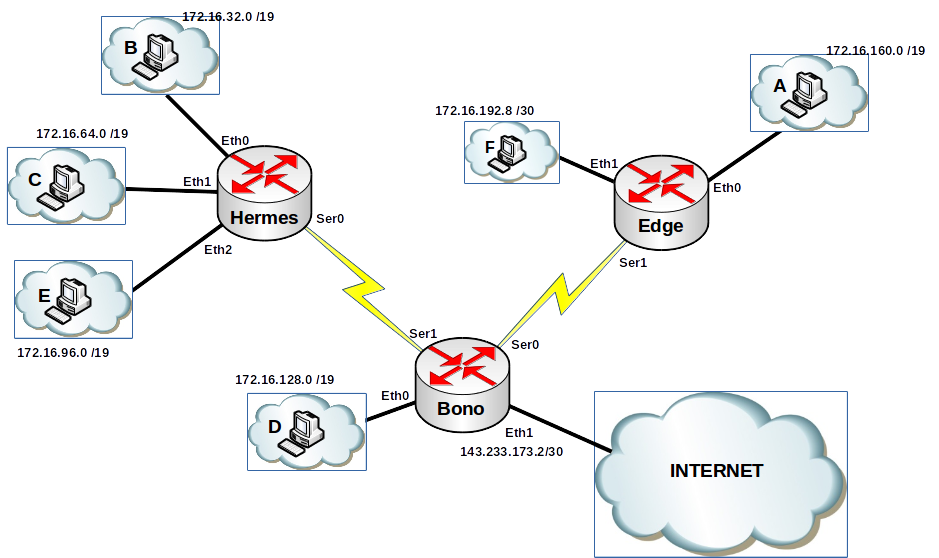
\includegraphics{images/lan.png}}
\end{center}
 
Παραδοτέα:

\begin{enumerate}
  \item Η έκθεση σας:
  \begin{enumerate}
     \item Screenshot της τοπολογίας.
     \item Screenshot που θα εμφανίζει τις επιτυχημένες προσπάθειες πρόσβασης 2 σταθμών στην υπηρεσία HTTP.
     \item Screenshot που θα αποδεικνύει το ζητούμενο 3, όπως διατυπώνεται παραπάνω.
     \item Screenshot με το αποτέλεσμα εκτέλεσης της εντολής \#show ip ospf
     \item Screenshot με το αποτέλεσμα εκτέλεσης της εντολής \#show ip ospf database
  \end{enumerate}
  \item Τα αρχεία (.pkt) με την τοπολογία σας.
\end{enumerate}

Ζητούμενα:


\section{Άσκηση 1η}
\subsection*{Εκφώνηση}

Screenshot της τοπολογίας.

\subsection*{Λύση}
\begin{center}
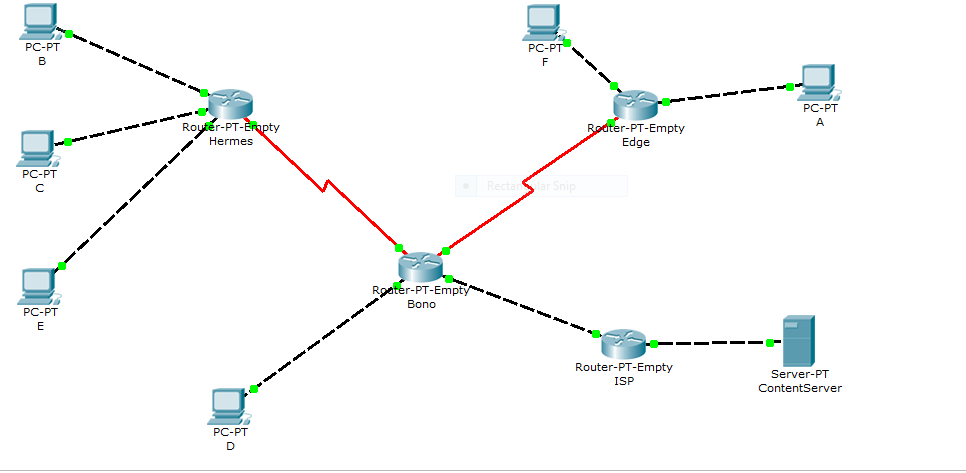
\includegraphics[width=\textwidth, height=\textheight, keepaspectratio]{images/topology.png}
\end{center}

\section{Άσκηση 2η}
\subsection*{Εκφώνηση}
Screenshot που θα εμφανίζει τις επιτυχημένες προσπάθειες πρόσβασης 2 σταθμών στην υπηρεσία HTTP.

\subsection*{Λύση}
Για να είναι δυνατή η πρόσβαση των σταθμών στον στην υπηρεσία http και μόνο σε
αυτή, εφαρμόστηκε στο interface Fa8/0 του Bono η εξής ACL:
\captionof{listing}{ACL για το β'}
\begin{minted}[breaklines=true, frame=lines, framesep=2mm, baselinestretch=1.2, fontsize=\footnotesize, linenos]{bash}
permit tcp any any eq www
\end{minted}

Ακολουθούν screenshot από επιτυχημένες προσπάθειες δύο σταθμών στην υπηρεσία
http.
\begin{center}
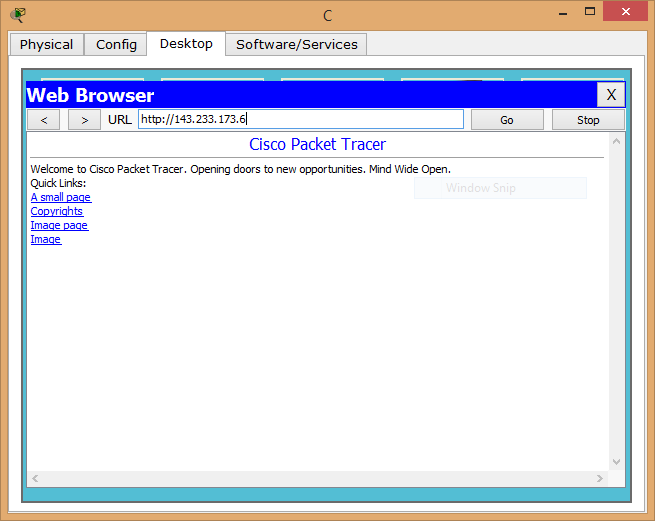
\includegraphics[width=\textwidth, height=\textheight, keepaspectratio]{images/http1.png}
\end{center}

\begin{center}
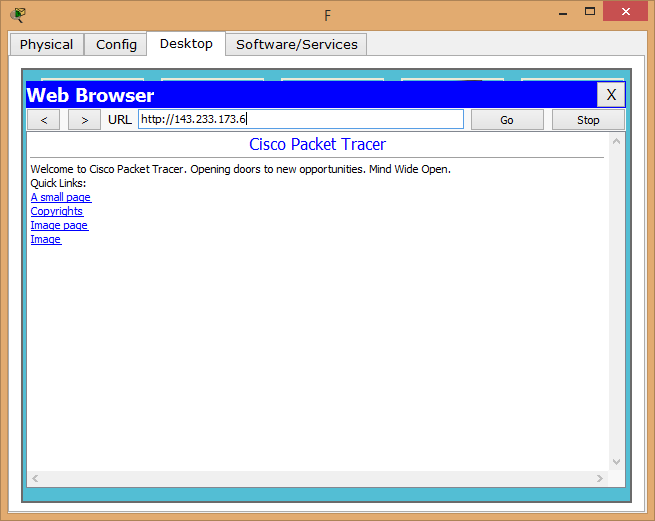
\includegraphics[width=\textwidth, height=\textheight, keepaspectratio]{images/http2.png}
\end{center}

\section{Άσκηση 3η}
\subsection*{Εκφώνηση}

Τα δίκτυα που βρίσκονται στον δρομολογητή Hermes είναι προσβάσιμα σε όλους τους άλλους μόνο σε περίπτωση χρήσης των εργαλείων ping και traceroute.

\subsection*{Λύση}
Σχετικά με το ζητούμενο 3, θέλουμε τα δίκτυα πίσω από τον Hermes να είναι
προσβάσιμα από τους άλλους μόνο για τις υπηρεσίες ping και traceroute. Συνεπώς,
εφαρμόζουμε στα interface Fa6/0, Fa7/0 και Fa8/0 την ACL:

\captionof{listing}{ACL για το γ'}
\begin{minted}[breaklines=true, frame=lines, framesep=2mm, baselinestretch=1.2, fontsize=\footnotesize, linenos]{bash}
permit icmp any any
\end{minted}

Όμως, εάν η ACL έμενε όπως παραπάνω θα υπήρχε το εξής πρόβλημα: Εάν κάποιο
από τα τερματικά πίσω από τον Hermes ήθελε να έχει πρόσβαση στις υπηρεσίες
HTTP του διαδικτύου ναι μεν η αίτηση του θα έφτανε στον ContentServer, αλλά
η απάντηση του Server θα αποριπτόταν από τον δρομολογητή Hermes καθώς επιτρέπει
μόνο εισερχόμενη κυκλοφορία ICMP. Για να λυθεί αυτό το πρόβλημα, και παράλληλα
να ισχύει το ζητούμενο 3, στα παραπάνω interface προστέθηκε και το παρακάτω
φίλτρο στην ACL:
\captionof{listing}{ACL για το γ' (2)}
\begin{minted}[breaklines=true, frame=lines, framesep=2mm, baselinestretch=1.2, fontsize=\footnotesize, linenos]{bash}
permit tcp any any established
\end{minted}
Με το παραπάνω επιτρέπονται τα tcp πακέτα προς τα τερματικά πίσω απο τον Hermes,
αλλά μόνο από επικοινωνία που έχουν ξεκινήσει αυτά τα τερματικά.

Σε ότι αφορά την απόδειξη, στα screenshot της προηγούμενης φαίνεται επιτυχημένο
http request από τερματικό του Hermes. Τέλος, στα δύο screenshot που ακολουθούν
φαίνεται επιτυχημένο ping request προς τερματικό του Hermes, καθώς και
μπλοκαρισμένο πακέτο tcp από επικοινωνία που έχει ξεκινήσει από τερματικό
εκτός του δικτύου Hermes. To τελευταίο επιτεύχθηκε με την λειτουργία simulation
του Packet Tracer.
\begin{center}
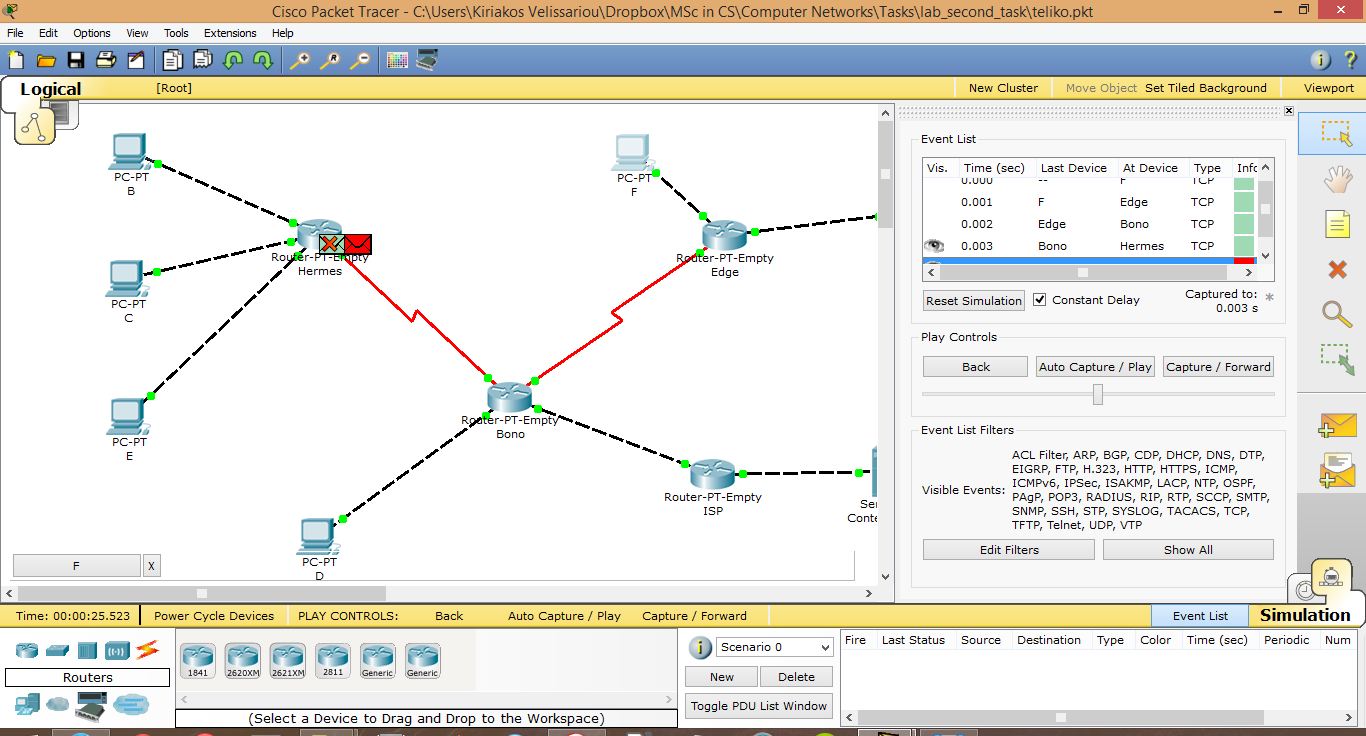
\includegraphics[width=\textwidth, height=\textheight, keepaspectratio]{images/third.png}
\end{center}
\begin{center}
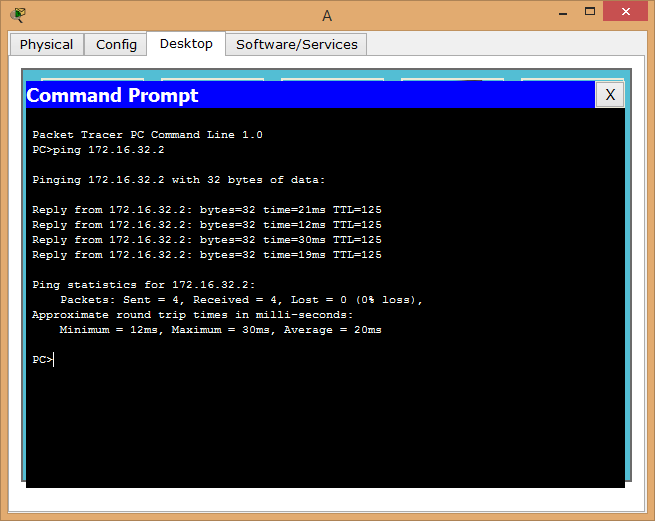
\includegraphics[width=\textwidth, height=\textheight, keepaspectratio]{images/third2.png}
\end{center}

\section{Άσκηση 4η}
\subsection*{Εκφώνηση}

Οι δρομολογητές αξιοποιούν τον αλγόριθμο OSPF για τη διαδικασία της δρομολόγησης. 
Προς το Διαδίκτυο χρησιμοποιείται στατική δρομολόγηση.

\subsection*{Λύση}

\captionof{listing}{Οι εντολές για το OSPF στον Hermes}
\begin{minted}[breaklines=true, frame=lines, framesep=2mm, baselinestretch=1.2, fontsize=\footnotesize, linenos]{bash}
Hermes(config)# router ospf 500
Hermes(config-router)# network 172.16.32.0 0.0.31.255 area 0
Hermes(config-router)# network 172.16.64.0 0.0.31.255 area 0
Hermes(config-router)# network 172.16.96.0 0.0.31.255 area 0
Hermes(config-router)# network 172.16.192.0 0.0.0.3 area 0
Hermes(config-router)# ^Z
Hermes(config)# ip route 143.233.173.0 255.255.255.252 172.16.192.1
\end{minted}

\captionof{listing}{Οι εντολές για το OSPF στον Edge}
\begin{minted}[breaklines=true, frame=lines, framesep=2mm, baselinestretch=1.2, fontsize=\footnotesize, linenos]{bash}
Edge(config)# router ospf 500
Edge(config-router)# network 172.16.192.8 0.0.0.3 area 0
Edge(config-router)# network 172.16.160.0 0.0.31.255 area 0
Edge(config-router)# network 172.16.192.4 0.0.0.3 area 0
Edge(config-router)# ^Z
Edge(config)# ip route 143.233.173.0 255.255.255.252 172.16.192.6
\end{minted}

\captionof{listing}{Οι εντολές για το OSPF στον Bono}
\begin{minted}[breaklines=true, frame=lines, framesep=2mm, baselinestretch=1.2, fontsize=\footnotesize, linenos]{bash}
Bono(config)# router ospf 500
Bono(config-router)# network 172.16.128.0 0.0.31.255 area 0
Bono(config-router)# network 172.16.192.0 0.0.0.3 area 0
Bono(config-router)# network 172.16.192.4 0.0.0.3 area 0
\end{minted}

\phantomsection \label{Βιβλιογραφία}
\addcontentsline{toc}{section}{Βιβλιογραφία}
%\mtcaddchapter[Βιβλιογραφία] % Λόγω του minitoc
\bibliographystyle{plain}
\bibliography{references}

\newpage

\end{document}

